% Sections/01_introduction.tex
% Introduction Section

\section{Introduction}
\label{sec:intro}

Human Activity Recognition (HAR) categorizes physical activities from sensor data to facilitate applications such as fall detection and fitness tracking. The UCI HAR dataset, a standard for the task, has 10,299 instances of six activities from accelerometer and gyroscope measurements on smartphones of 30 subjects, providing dense, multi-dimensional data for centralized learning and distributed learning~\cite{anguita2013public}.

Whereas conventional centralized approaches gather all the information in a single hub—creating privacy and regulative issues—Federated Learning (FL) supports decentralized training with data stored locally on user devices and model updates only shared~\cite{mcmahan2017communication}. This is naturally appropriate to HAR, where sensor signals are inherently personal and spread out. This paper illustrates that FL, when paired with differential privacy, both ensures user privacy and retains high accuracy. It analyzes privacy–utility trade-offs in federated and centralized settings and sets the basis for scalable, privacy-aware HAR applications deployable on personal devices~\cite{abadi2016deep}.

\begin{figure}[htbp]
  \centering
  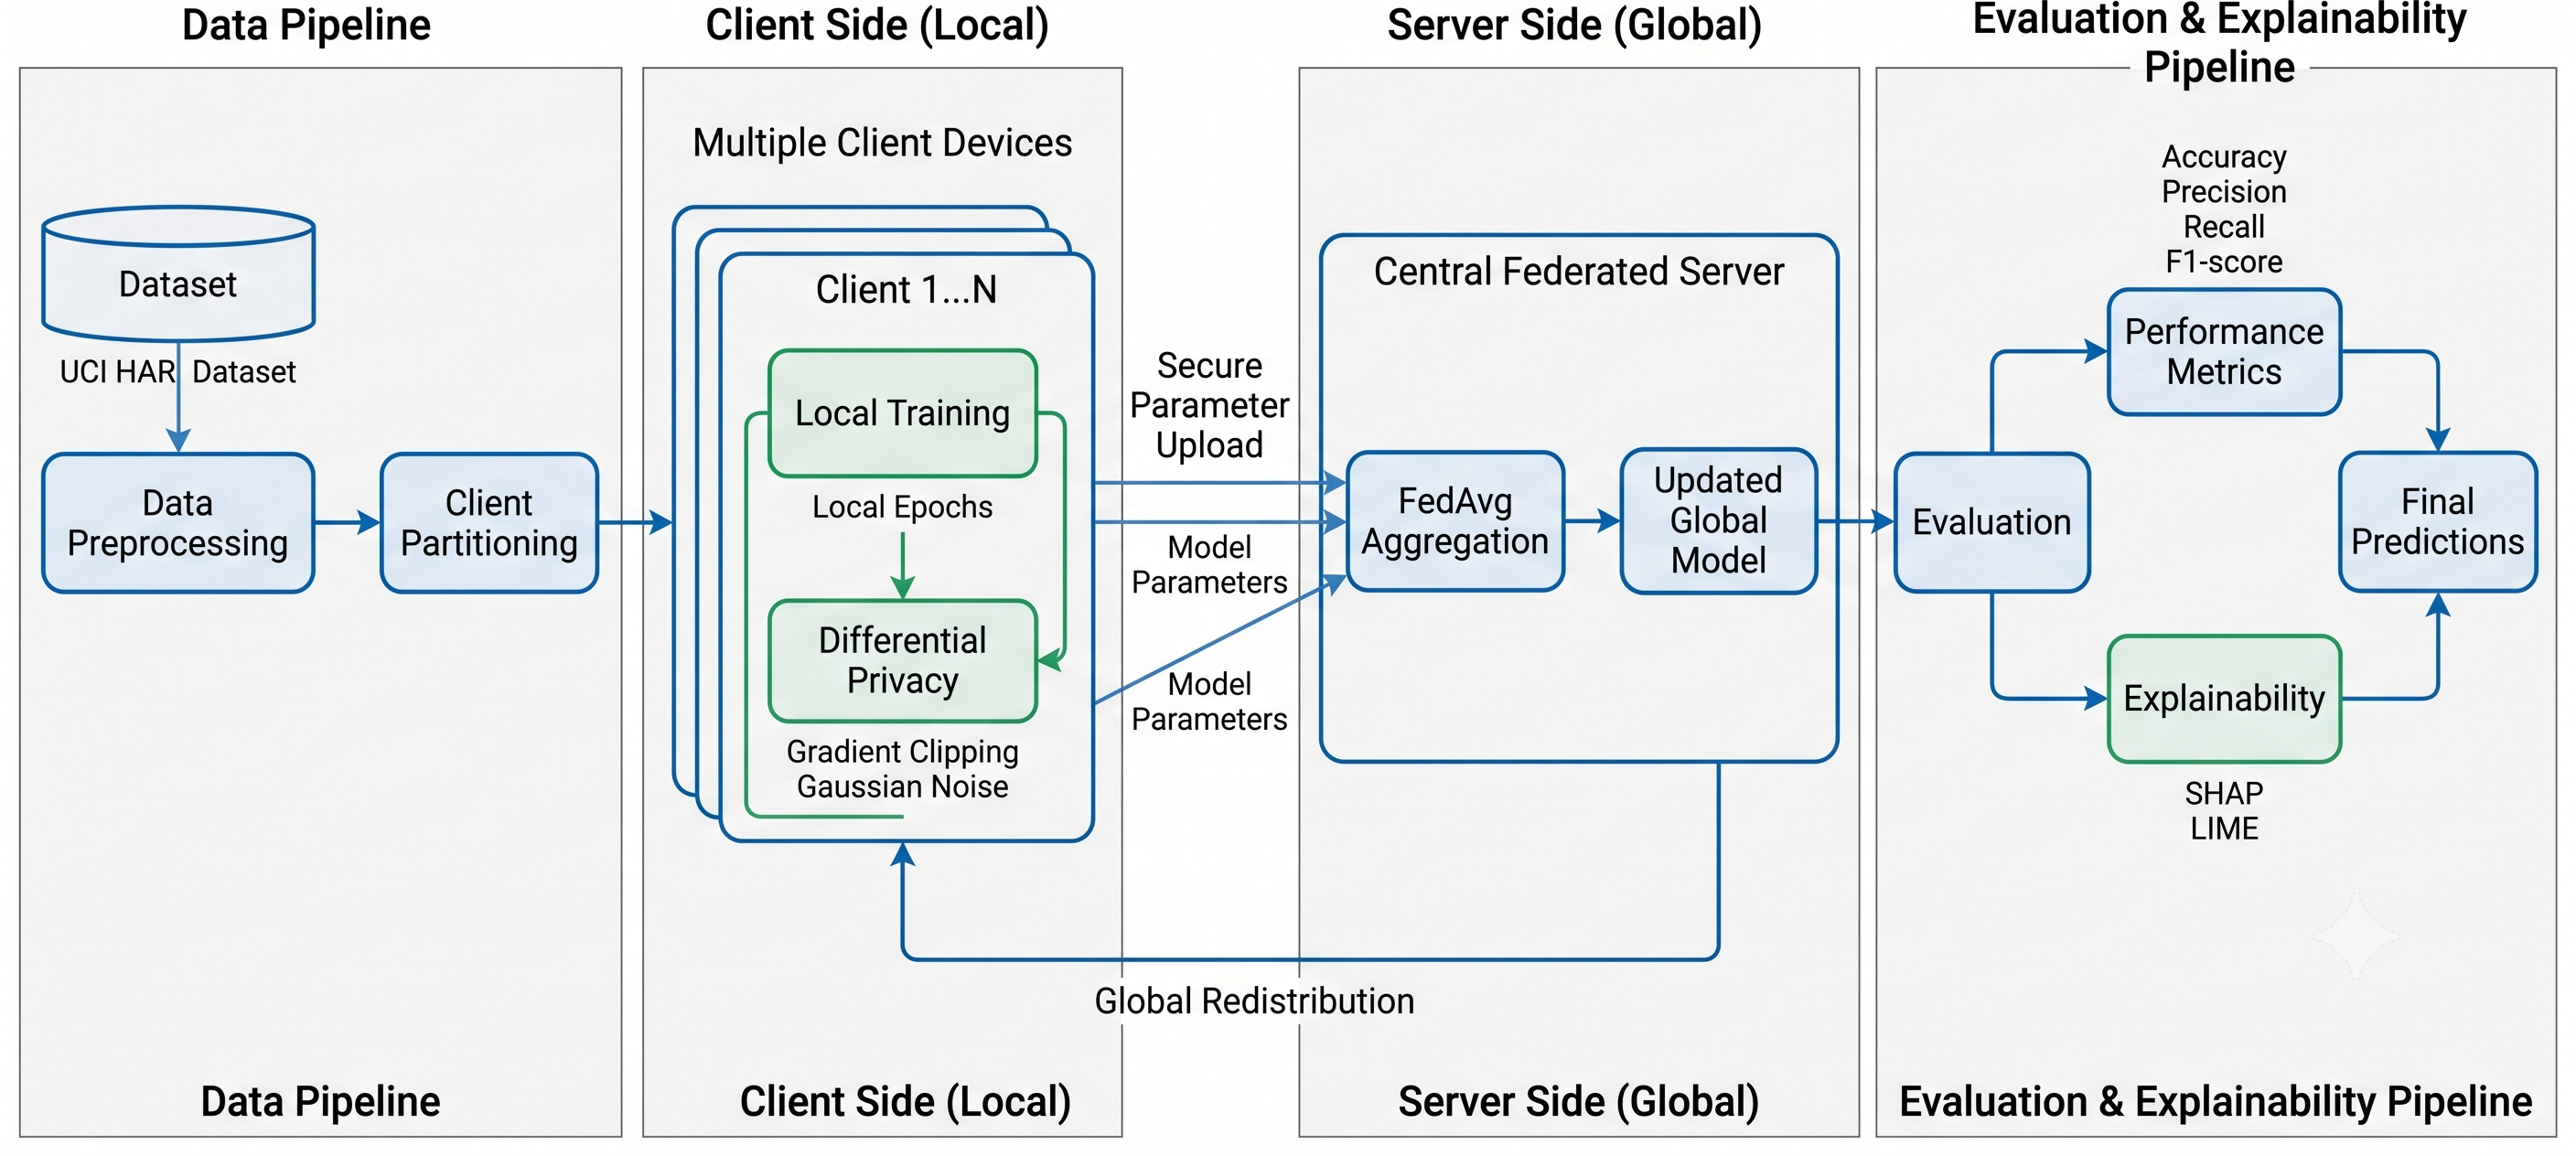
\includegraphics[width=\textwidth]{figures/fig1.png}
  \caption{Client-Level Differentially Private Federated Learning architecture.}
  \label{fig:architecture}
\end{figure}

Schematic shows how a federated model with a central server coordinates and processes encrypted updates from each linked devices through a global, common training model after locally training them on activities like walking or cycling. Raw, personal data remains on devices securely, protects user privacy and enable collaborative model improvement with iterative communication rounds.
